\documentclass[journal]{vgtc}                % final (journal style)
%\documentclass[review,journal]{vgtc}         % review (journal style)
%\documentclass[widereview]{vgtc}             % wide-spaced review
%\documentclass[preprint,journal]{vgtc}       % preprint (journal style)
%\documentclass[electronic,journal]{vgtc}     % electronic version, journal

%% Uncomment one of the lines above depending on where your paper is
%% in the conference process. ``review'' and ``widereview'' are for review
%% submission, ``preprint'' is for pre-publication, and the final version
%% doesn't use a specific qualifier. Further, ``electronic'' includes
%% hyperreferences for more convenient online viewing.

%% Please use one of the ``review'' options in combination with the
%% assigned online id (see below) ONLY if your paper uses a double blind
%% review process. Some conferences, like IEEE Vis and InfoVis, have NOT
%% in the past.

%% Please note that the use of figures other than the optional teaser is not permitted on the first page
%% of the journal version.  Figures should begin on the second page and be
%% in CMYK or Grey scale format, otherwise, colour shifting may occur
%% during the printing process.  Papers submitted with figures other than the optional teaser on the
%% first page will be refused.

%% These three lines bring in essential packages: ``mathptmx'' for Type 1
%% typefaces, ``graphicx'' for inclusion of EPS figures. and ``times''
%% for proper handling of the times font family.

\usepackage{mathptmx}
\usepackage{graphicx}
\usepackage{times}
\usepackage{epstopdf}

%% We encourage the use of mathptmx for consistent usage of times font
%% throughout the proceedings. However, if you encounter conflicts
%% with other math-related packages, you may want to disable it.

%% This turns references into clickable hyperlinks.
\usepackage[bookmarks,backref=true,linkcolor=black]{hyperref} %,colorlinks
\hypersetup{
  pdfauthor = {},
  pdftitle = {},
  pdfsubject = {},
  pdfkeywords = {},
  colorlinks=true,
  linkcolor= black,
  citecolor= black,
  pageanchor=true,
  urlcolor = black,
  plainpages = false,
  linktocpage
}

%% If you are submitting a paper to a conference for review with a double
%% blind reviewing process, please replace the value ``0'' below with your
%% OnlineID. Otherwise, you may safely leave it at ``0''.
\onlineid{0}

%% declare the category of your paper, only shown in review mode
\vgtccategory{Research}

%% allow for this line if you want the electronic option to work properly
\vgtcinsertpkg

%% In preprint mode you may define your own headline.
%\preprinttext{To appear in an IEEE VGTC sponsored conference.}

%% Paper title.

\title{Global Illumination for Fun and Profit}

%% This is how authors are specified in the journal style

%% indicate IEEE Member or Student Member in form indicated below
\author{Roy G. Biv, Ed Grimley, \textit{Member, IEEE}, and Martha Stewart}
\authorfooter{
%% insert punctuation at end of each item
\item
 Roy G. Biv is with Starbucks Research. E-mail: roy.g.biv@aol.com.
\item
 Ed Grimley is with Grimley Widgets, Inc.. E-mail: ed.grimley@aol.com.
\item
 Martha Stewart is with Martha Stewart Enterprises at Microsoft
 Research. E-mail: martha.stewart@marthastewart.com.
}

%other entries to be set up for journal
\shortauthortitle{Biv \MakeLowercase{\textit{et al.}}: Global Illumination for Fun and Profit}
%\shortauthortitle{Firstauthor \MakeLowercase{\textit{et al.}}: Paper Title}

%% Abstract section.
\abstract{Visualizations of biological structures across multiple scales are becoming popular as more and more detailed data from the atomic level up to the cellular level are becoming available. To support seamless interactive exploration of such models, visual representations of elements on different levels of detail are necessary. While multi-scale structural representations have been extensively explored in the past (?), we address a new challenge introduced in multi-scale visualizations covering several orders of magnitude, namely multi-scale color coding. Categorical color coding is essential for identification of structures, but their usage varies with the level of detail from the visualization, from encoding atom types to compartments of a cell. 
} % end of abstract

%% Keywords that describe your work. Will show as 'Index Terms' in journal
%% please capitalize first letter and insert punctuation after last keyword
\keywords{Radiosity, global illumination, constant time}

%% ACM Computing Classification System (CCS). 
%% See <http://www.acm.org/class/1998/> for details.
%% The ``\CCScat'' command takes four arguments.

\CCScatlist{ % not used in journal version
 \CCScat{K.6.1}{Management of Computing and Information Systems}%
{Project and People Management}{Life Cycle};
 \CCScat{K.7.m}{The Computing Profession}{Miscellaneous}{Ethics}
}

%% Uncomment below to include a teaser figure.
  \teaser{
 \centering
 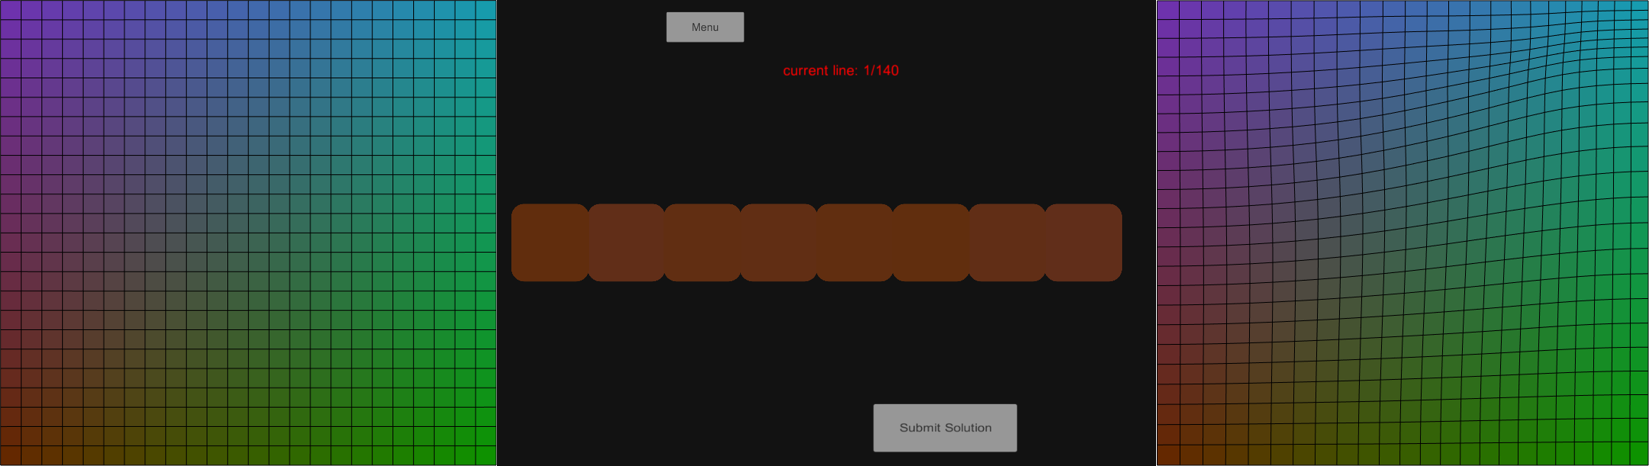
\includegraphics[width=16cm]{Picture1}
  \caption{In the Clouds: Vancouver from Cypress Mountain.}
  }

%% Uncomment below to disable the manuscript note
%\renewcommand{\manuscriptnotetxt}{}

%% Copyright space is enabled by default as required by guidelines.
%% It is disabled by the 'review' option or via the following command:
% \nocopyrightspace

%%%%%%%%%%%%%%%%%%%%%%%%%%%%%%%%%%%%%%%%%%%%%%%%%%%%%%%%%%%%%%%%
%%%%%%%%%%%%%%%%%%%%%% START OF THE PAPER %%%%%%%%%%%%%%%%%%%%%%
%%%%%%%%%%%%%%%%%%%%%%%%%%%%%%%%%%%%%%%%%%%%%%%%%%%%%%%%%%%%%%%%%

\begin{document}

%% The ``\maketitle'' command must be the first command after the
%% ``\begin{document}'' command. It prepares and prints the title block.

%% the only exception to this rule is the \firstsection command
\firstsection{Introduction}

\maketitle

%% \section{Introduction} %for journal use above \firstsection{..} instead

Biological organisms can be viewed on different scales. For example, the human body consists of organs, cells, proteins and molecules. As more detailed data is becoming available across all levels, it is possible to combine visualizations of multiple scale levels into a single integrated visual environment. This poses new challenges for visualization experts, including seamlessly adapting the levels of detail of structural representations for real-time rendering, .... (experts, please address the challenges). \newline
A challenge which has not been addressed so far is color-coding. Consider, for instance, the human immunodeficiency virus (HIV). To understand its viral lifecycle, researchers are investigating the shape of its compartments, the role of the individual proteins in viral replication, the secondary structures, as well as structural properties of binding sites on the atomic level. Traditionally, researchers use dedicated visual representations for each level of scale, and illustrators provide hand-crafted visualizations to communicate new findings to the general public. Each of these scale levels uses a distinct color coding so that observers are able to distinguish and identify the structures. Can we show existing examples here? \newline
When integrating multiple scales into a single zoomable visualization, it is therefore necessary to not only provide a seamless structural zooming, but also a color-coding mechanism that takes the current level of detail into account. While successively providing more levels of detail of the structures when zooming in, we are severely limited in the number of available colors due to perceptual constraints and limitations of the monitor hardware. \newline

We propose a semantic zooming method for visualizing color-coded a virusmulti-scale visualization based on a view- dependent hierarchical color-scheme. Starting from the lowest zoom-level, we iteratively split up the available color space to the number of necessary colors defined by the current zoom level and item visibility. Our method thereby trades discriminability of individual elements against temporal coherence. In the HIV example (refer to teaser image), the user initially sees the different compartments. As the user zooms in, the proteins receive more distinct colors based on which compartment they are in. As compartments and proteins disappear, the colors of the visible proteins are adjusted to enhance discernibility.  As the viewer zooms further in, the domains of the proteins will become distinct, and eventually even the atoms, whose colors are predefined by convention. 



\section{Related Work}

Color maps are used often in visualization. Their structure depends heavily on the application, as has been shown in [Colour for Presentation Graphics], [Color Design for Illustrative Visualization], A Rule-based Tool for Assisting Colormap Selection, http://ultra.sdk.free.fr/docs/Image/Colors/ARule-basedToolfo0AssistingColormapSelection.htm], [Choosing Effective Colours for Data Visualization], [a survey and task-based quality assessment of static 2d colormaps], [explorative analysis of 2d color maps]. Several tools have been developed to assist users select appropriate color maps, such as colorbrewer, or iwanthue, [http://tools.medialab.sciences-po.fr/iwanthue/] and XCluSim, which are aimed at generating colors for clusters of data. Such clustering can, however, cause perceptual issues, either due to the large number of clusters or their layout. Particular care needs to be taken when dealing with higher dimensional data [revisiting perceptually optimized color mapping for high dimensional data analysis], so the distances between the clusters do not become distorted. Furthermore, in cases such as coloring maps, visually dominant structures may visually suppress small groups or areas [Perceptually Driven Visibility Optimization for Categorical Data Visualization]. Recognition may also be affected by contrast effects which may need to be dealt with [Methods for Compensating Contrast Effects in Information Visualization].
XCluSim’s uses a tree based method [tree based method] that attempts to overcome these issues in the case of hierarchical structures. The tree method uses HCL space – a cylindrical coordinate version of CIELab with Hue , Chroma (Saturation), and Luminance – and gives each cluster a different hue. The root of the tree has no chroma, i.e. grey, and the hue is divided up into different sections, one for each branch, with some space cut out between branches, in order for there to be a jump in color from one section to another. As the tree spreads out, the chroma of the nodes increases, and each level gets its own smaller subsection. 
Sometimes hierarchical data can also be viewed on multiple levels at once, for example a protein can be viewed on the overall structure as well as on the atomic structure [Rendering Molecular Surfaces using Order-Independent Transparency]. Alternatively, distortions of the object or different rendering levels in different areas of the camera may be used. For example, in [A Rendering Framework for Multiscale Views of 3D Models] the area in the center of the camera is rendered as closer in. This is achieved through…. . Parts of the object can also be distorted, by example through widgets such as in [Non-linear perspective widgets for creating multiple-view images] or [Vessel visualization using curvicircular feature aggregation]. In the first case X, in the second case Y.



Level of detail and abstraction may also depend on the distance from the object.[ View-dependent level-of-detail abstraction for interactive atomistic visualization of biological struct] [Illustrative Molecular Visualization with Continuous Abstraction] [Illustrating the Machinery of Life: Viruses Continuous Levels-of-Detail and Visual Abstraction for Seamless Molecular Visualization]. 
These kinds of visualizations have to deal with two major problems. First is when to show which level and how many levels to show at once. An example of this is [A Rendering Framework for Multiscale Views of 3D Models] by x, where they show a method of showing different levels of detail of a human body. In our case, we don’t want to allow for distortion, as most of the items are a) fairly small, b) should be comparable to other elements nearby without distortion, and c) the user does not want to see all layers at once, as the structure of a protein holds little information about the structure of a cell.


\begin{table}
%% Table captions on top in journal version
 \caption{SciVis Paper Acceptance Rate: 1994-2006}
 \label{vis_accept}
 \scriptsize
 \begin{center}
   \begin{tabular}{cccc}
     Year & Submitted & Accepted & Accepted (\%)\\
   \hline
     1994 &  91 & 41 & 45.1\\
     1995 & 102 & 41 & 40.2\\
     1996 & 101 & 43 & 42.6\\
     1997 & 117 & 44 & 37.6\\
     1998 & 118 & 50 & 42.4\\
     1999 & 129 & 47 & 36.4\\
     2000 & 151 & 52 & 34.4\\
     2001 & 152 & 51 & 33.6\\
     2002 & 172 & 58 & 33.7\\
     2003 & 192 & 63 & 32.8\\
     2004 & 167 & 46 & 27.6\\
     2005 & 268 & 88 & 32.8\\
     2006 & 228 & 63 & 27.6
   \end{tabular}
 \end{center}
\end{table}

\begin{figure}[htb]
 \centering
 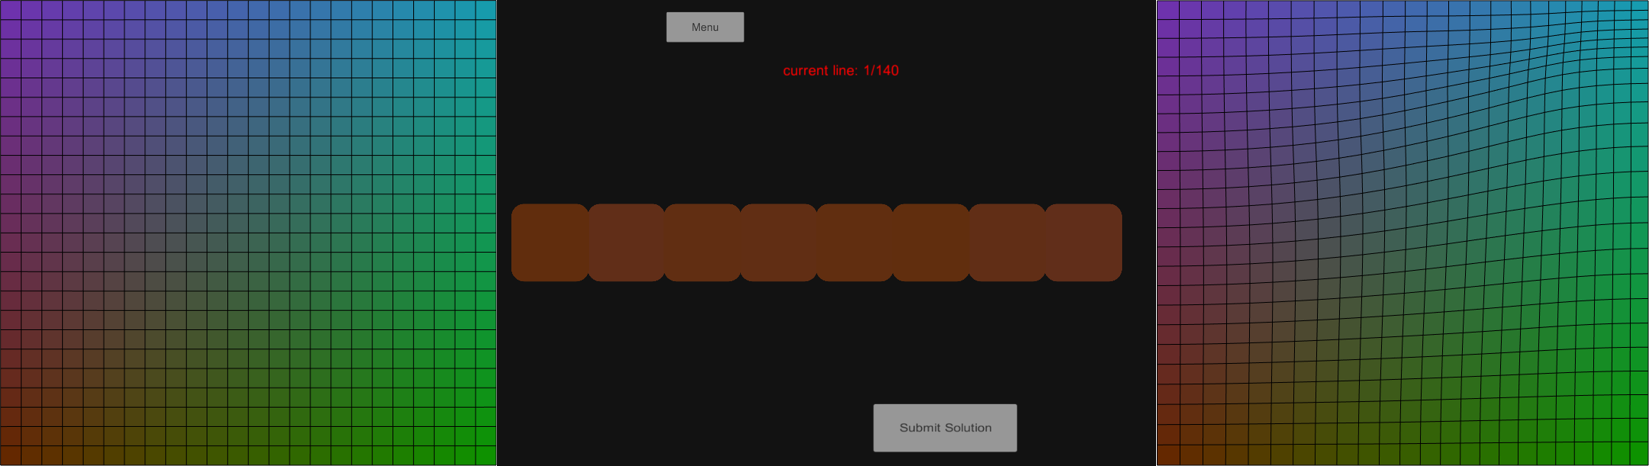
\includegraphics[width=1.5in]{Picture1}
 \caption{Sample illustration.}
\end{figure}

\subsection{Mezcal Head}

Duis autem~\cite{Lorensen:1987:MCA} vel eum iriure dolor in hendrerit
in vulputate velit esse molestie consequat, vel illum dolore eu
feugiat nulla facilisis at vero eros et accumsan et iusto odio
dignissim qui blandit praesent luptatum zzril delenit augue duis
dolore te feugait nulla facilisi. Lorem ipsum dolor sit amet,
consectetuer adipiscing elit, sed diam nonummy nibh euismod tincidunt
ut laoreet dolore magna aliquam erat volutpat%
\footnote{Footnotes appear at the bottom of the column}.


\subsubsection{Ejector Seat Reservation}

Ut wisi enim ad minim veniam, quis nostrud exerci tation ullamcorper
suscipit lobortis nisl ut aliquip ex ea commodo
consequat~\cite{Nielson:1991:TAD}. Duis autem vel eum iriure dolor in
hendrerit in vulputate velit esse molestie consequat, vel illum dolore
eu feugiat nulla facilisis at vero eros et accumsan et iusto odio
dignissim qui blandit praesent luptatum zzril delenit augue duis
dolore te feugait nulla facilisi.

\paragraph{Rejected Ejector Seat Reservation}

Ut wisi enim ad minim veniam, quis nostrud exerci tation ullamcorper
suscipit lobortis nisl ut aliquip ex ea commodo consequat. Duis autem
vel eum iriure dolor in hendrerit in vulputate velit esse molestie

\section{Conclusion}

Lorem ipsum dolor sit amet, consetetur sadipscing elitr, sed diam
nonumy eirmod tempor invidunt ut labore et dolore magna aliquyam erat,
sed diam voluptua. At vero eos et accusam et justo duo dolores et ea
rebum. Stet clita kasd gubergren, no sea takimata sanctus est Lorem
ipsum dolor sit amet. Lorem ipsum dolor sit amet, consetetur
sadipscing elitr, sed diam nonumy eirmod tempor invidunt ut labore et
dolore magna aliquyam erat, sed diam voluptua. At vero eos et accusam
et justo duo dolores et ea rebum. Stet clita kasd gubergren, no sea
takimata sanctus est Lorem ipsum dolor sit amet. Lorem ipsum dolor sit
amet, consetetur sadipscing elitr, sed diam nonumy eirmod tempor
invidunt ut labore et dolore magna aliquyam erat, sed diam
voluptua. At vero eos et accusam et justo duo dolores et ea
rebum. Stet clita kasd gubergren, no sea takimata sanctus est Lorem
ipsum dolor sit amet.

Lorem ipsum dolor sit amet, consetetur sadipscing elitr, sed diam
nonumy eirmod tempor invidunt ut labore et dolore magna aliquyam erat,
sed diam voluptua. At vero eos et accusam et justo duo dolores et ea
rebum. Stet clita kasd gubergren, no sea takimata sanctus est Lorem
ipsum dolor sit amet. Lorem ipsum dolor sit amet, consetetur
sadipscing elitr, sed diam nonumy eirmod tempor invidunt ut labore et
dolore magna aliquyam erat, sed diam voluptua. At vero eos et accusam
et justo duo dolores et ea rebum. 

%% if specified like this the section will be committed in review mode
\acknowledgments{
The authors wish to thank A, B, C. This work was supported in part by
a grant from XYZ.}

\bibliographystyle{abbrv}
%%use following if all content of bibtex file should be shown
%\nocite{*}
\bibliography{template}
\end{document}
